
This section might be redundant with what has been said in the course, nevertheless, it gives a quick view of what the document is about.

Zookeeper is a service for coordinating processes of distributed applications. The core design principle of Zookeeper is to not implement services for each different coordination needs (called primitives) but instead to it exposes an API that enable the development of such primitives. This lead to the implementation of a \textbf{coordination kernel} that enables new primitives without requiring changes to the service core.

\subsection{Zookeeper service}

Before going further a little terminology might be of use:
\begin{itemize}
\item \textbf{Client}: user of Zookeeper service.
\item \textbf{Server}: process providing the Zookeper service.
\item \textbf{Znode}: in-memory data node in the Zookeeper data.
\item \textbf{Session}: a client connects to Zookeeper and initiates a session. The session ends when the client explicitly close a session handle or Zookeeper detects the client as faulty (through a session-timeout $\Leftrightarrow$ the client hasn't send anything for a given time)
\end{itemize}

Znodes can be further divided : 

\begin{itemize}
	\item \textbf{regular}: clients manipulate regular znodes by creating and deleting them explicitly.
	\item \textbf{ephemeral}: clients can delete them explicitly or let the system remove them automatically when their session terminates.
\end{itemize}

\begin{figure}
	\begin{center}
		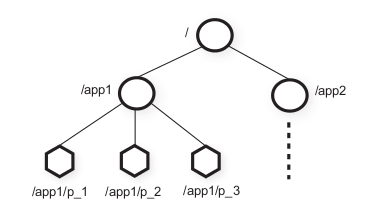
\includegraphics[scale=1]{img/hierachicalZookeeper.png}
	\end{center}
	\caption{Illustration of ZooKeeper hierarchical name space}
	\label{hierarchicalname}
\end{figure}

Znodes are organized according to a hierarchical name space. It is roughly the same as for a file system, see figure \ref{hierarchicalname}. The nodes in this hierarchy are data objects that clients manipulate through the ZooKeeper API. All znodes store data, and all znodes, except for ephemeral znodes, can have children.

When creating a new znode, a client can set the \textbf{sequential flag}: Nodes created with this flag set have the value of a monotonically increasing counter appended to its name.

When a client wants to have notifications of changes done on some data. This is done through watches, when the client issues a read operation, the operation completes as normal but the server promises to notify the client when the information returned has changes. Watches are one-time trigger.



\subsection{Guarantees}
Zookeeper has two basic ordering guarantees: 
\begin{itemize}
\item \textbf{Linearizable writes}: all requests that update the state of Zookeeper are serializable and respect precedence. This is assured through the leader-based atomic broadcast protocol called Zab
\item \textbf{FIFO client order}: all requests from a given client are executed in the order that the were sent by the client.
\end{itemize}

The paper also focuses on some problem that can arise in certain circumstances, go and see section 2.3 of the document (it is done with an example).

Zookeeper adds two other guarantees:
\begin{itemize}
\item \textbf{liveness}: if a majority of Zookeeper servers are active and communicating the service will be available
\item \textbf{durability}: if ZooKeeper responds successfully to a change request, that change persists across any number of failures as long a a quorum of servers ($\approx$ majority) is eventually able to recover.
\end{itemize}

The paper also focuses on examples of primitives implementations see section 2.4.
\subsection{Zookeeper Implementation}

When a client sends a write request, it is forwarded to a single server called the leader The rest of the ZooKeeper servers, called followers, receive message proposals consisting of state changes from the leader and agree upon state changes. In fact the leader executes the request and then broadcast the change to the ZooKeeper state through Zab, an atomic broadcast protocol.

Going from the request of the client to the changes of the ZooKeeper state is done using transactions. When a leader receives a write request, it calculates what the state of the system will be when the write is applied and transforms it into a transaction that captures this new state.

Transactions are idempotent, meaning that applying this transaction one or several times won't make any difference.


